% $Id$
\documentclass[11pt]{article}
\usepackage{epsfig}
\usepackage{dcolumn}

\def\numpackages{27}
\def\numlines{1.2 million}

\newcommand{\pkg}[1]{\textsf{#1}}

% the "fullpage" package does almost the same thing
% as the below lines-- it doesn't make things quite as
% tall or wide, but is generally what I use
% \usepackage{fullpage}
\marginparwidth 0pt
\oddsidemargin  0pt
\evensidemargin 0pt
\marginparsep 0pt
\topmargin   0pt
\textwidth   6.5 in
\textheight  8.5 in

\renewcommand{\floatpagefraction}{.8} %default .5
% Avoid putting all figures at end of text.
\renewcommand{\textfraction}{.1}  % .2 is the default
\renewcommand{\topfraction}{.9}   % .7 is the default

\begin{document}
% \bibliographystyle{plain}
\bibliographystyle{alpha}

\title{An Empirical Analysis of C Preprocessor Use}

\author{Michael D. Ernst%
  \and Greg J. Badros%
  \thanks{Supported by a National Science Foundation
    Graduate Fellowship. Any opinions, findings, conclusions, or
    recommendations expressed in this publication are those of the
    author, and do not necessarily reflect the views of the National
    Science Foundation.}
  \and David Notkin}

\date{Technical Report UW-CSE-97-04-06 \\
Department of Computer Science and Engineering \\
University of Washington \\
Box 352350, Seattle, WA  98195-2350  USA \\
{\small \{{\tt mernst},{\tt gjb},{\tt notkin}\}{\tt @cs.washington.edu}} \\
22 April 1997}  

\maketitle

\begin{abstract}

  The C programming language is intimately connected to its macro
  preprocessor.  This relationship affects, indeed generally hinders, both
  the tools (compilers, debuggers, call graph extractors, etc.)\ built to
  engineer C programs and also the ease of translating to other languages
  such as C++.  This paper analyzes {\numpackages} packages comprising
  {\numlines} lines of publicly available C code, determining how
  the preprocessor is used in practice.  We developed a framework for
  analyzing preprocessor usage and used it to extract information about the
  incidence of preprocessor directives, the frequency of macro use and
  redefinition, the purposes of macros (in terms of both definitions and
  uses), and expressibility of macros in terms of other C or C++
  language features.  We particularly note
  data that are material to the development of tools for C or C++,
  including translating from C to C++ to reduce preprocessor usage.
  The results are of interest to language designers, tool writers,
  programmers, and software engineers.
\end{abstract}

\bigskip

\section{Introduction}

The C programming language~\cite{ansi} is intimately connected to its
macro preprocessor, Cpp~\cite[Ch.~3]{Harbison91}.  In particular, the
preprocessor supplies essential facilities such as file inclusion,
definition of constants and macros, and conditional compilation; these
can be used to define new syntax, abbreviate repetitive or complicated
constructs, or eliminate reliance on a compiler implementation to
inline functions, propagate symbolic constants, eliminate dead code,
and short-circuit constant tests.  The latter guarantees are
especially valuable for compilers that do a poor job optimizing or
when the programmer wishes to override the compiler's heuristics.  Cpp
also permits system dependences to be made explicit and tested,
resulting in a clearer separation of concerns.  Finally, Cpp permits a
single source to contain multiple different dialects of C; a frequent
use is to support both K\&R-style and ANSI-style declarations.

Indeed, one cannot write practical C programs without these
facilities.  While disciplined use of the preprocessor can reduce
programmer effort and improve portability, performance, or
readability, Cpp also lends itself to arbitrary source code
manipulations that complicate understanding of the program by both
software engineers and tools.  The designer of C++, which shares C's
preprocessor, also noted these problems: ``Occasionally, even the most
extreme uses of Cpp are useful, but its facilities are so unstructured
and intrusive that they are a constant problem to programmers,
maintainers, people porting code, and tool
builders.''~\cite[p.~424]{Stroustrup-DesignEvolution}

Tools\,---\,and, to a lesser degree, software engineers\,---\,have
three options for coping with Cpp.  They may ignore preprocessor
directives altogether, accept only post-processed code (usually by
running Cpp on their input), or attempt to emulate the preprocessor.
Each approach has different strengths and weaknesses.

\begin{itemize}

\item Ignoring preprocessor directives is an option for approximate
tools (such as those based on lexical or approximate parsing
techniques).  However, if accurate information about function extents,
scope nesting, declared variables and functions, and other aspects of
a program are required, the preprocessor cannot be ignored.

\item Operating on post-processed code, the most common strategy, is
simple to implement, but then the tool's input differs from what the
programmer sees.  Even when line number mappings are maintained, other
information is lost in the mapping back to the original source code.
For instance, source-level debuggers have no symbolic names or types
for constants and functions introduced via {\tt \#define}, nor can
tools trace or set breakpoints in function macros, as they can for
ordinary functions (even those that have been
inlined~\cite{Zellweger83:TR}).  As another example, Siff and Reps
describe a technique that uses type inferencing to produce C++
function templates from C; however, the input is ``a C program
component that $\ldots$ has been preprocessed so that all include
files are incorporated and all macros
expanded~\cite[p.~145]{Siff-fse96}.''  Such preprocessing may limit
the readability and reusability of the resulting C++ templates.  As
yet another related example, call graph extractors generally work in
terms of the post-processed code, even when a human is the intended
consumer of the call graph~\cite{Murphy-icse18}.  Some tools even
leave the software engineer responsible for inferring the mapping
between the original and the post-processed source, which is an
undesirable and error-prone situation.

In addition, a tool that manipulates post-processed code cannot be run
on a non-syntactic program or one that will not preprocess on the
platform on which the tool is being run.  These constraints complicate
porting and maintenance, two of the situations in which program
understanding and transformation tools are most likely to be needed.
Additionally, a tool supplied with only one post-processed
instantiation of the source code cannot reason about the program as a
whole, only about that version that results from one particular set of
preprocessor variables.  For instance, a bug in one configuration may
not be discovered despite exhaustive testing of other configurations
that do not incorporate particular code or do not admit particular
execution paths.

\item The final option, emulating the preprocessor, is fraught with
difficulty.  Macro definitions consist of complete tokens but need not
be complete expressions or statements.  Conditional compilation and
alternative macro definitions lead to very different results from a
single original program text.  Preprocessing adds complexity to an
implementation, which must trade off performing preprocessing against
maintaining the code in close to its original form.  Extracting
structure from macro-obfuscated source is not a task for the
faint-hearted.  Despite these problems, in many situations only some
sort of preprocessing or Cpp analysis can produce useful answers.

\end{itemize}

To build a better understanding of how the preprocessor is used, with
the intent of helping tool builders select among these approaches, we
performed an analysis of preprocessor usage across {\numpackages} C
packages comprising {\numlines} lines of code.
Figure~\ref{fig:packages} describes the packages and lists their sizes
in terms of physical lines (or newline characters) and non-comment,
non-blank (NCNB) lines, which disregards lines consisting of only
comments or whitespace.  The remainder of the analysis reports in
terms of NCNB length.

\begin{figure}
\centering
{% ``\small'' here has no effect; in a table, each cell is its own group.
 % It will require a hack to make the table smaller as I'd like it.
  \setlength{\tabcolsep}{.25em}
  \begin{tabular}{|l|r|r|r|r|l|}\hline
Package & Version & Physical lines & NCNB lines & Files & Description\\\hline\hline
bash & 1.14.7 & 67,604 & 46,110 & 151 & Command shell \\\hline
bc & 1.03 & 7,483 & 5,184 & 28 & Desktop calculator \\\hline
bison & 1.25 & 11,434 & 7,676 & 33 & Parser generator \\\hline
cvs & 1.9 & 79,670 & 53,431 & 208 & Revision control system \\\hline
dejagnu & 1.3 & 64,650 & 40,286 & 150 & Testing framework \\\hline
emacs & 19.34 & 206,309 & 134,251 & 445 & Text editor\\\hline
flex & 2.5.3 & 18,969 & 13,289 & 32 & Scanner generator \\\hline
fvwm & 2.0.43 & 55,584 & 42,498 & 151 & Window manager \\\hline
g77 & 0.5.18 & 133,366 & 98,980 & 232 & Fortran compiler \\\hline
gawk & 2.15.6 & 27,705 & 18,567 & 61 & GAWK interpreter \\\hline
gcc & 2.7.2.1 & 500,752 & 324,620 & 706 & C and C++ compiler\\\hline
genscript & 1.3.2a & 12,049 & 8,166 & 32 & Text-to-PostScript converter \\\hline
ghostview & 1.5 & 11,535 & 8,897 & 23 & PostScript previewer \\\hline
gnuchess & 4.0pl77 & 30,090 & 18,538 & 41 & Chess player \\\hline
gnuplot & 3.50.1.17 & 38,209 & 29,582 & 59 & Graph plotter \\\hline
groff & 1.10 & 68,872 & 60,054 & 162 & Text formatter \\\hline
gs & 262 & 77,695 & 56,378 & 309 & PostScript interpreter \\\hline
gzip & 1.2.4 & 9,067 & 5,774 & 34 & File compressor \\\hline
m4 & 1.4 & 16,778 & 10,327 & 28 & Macro expander \\\hline
mosaic & 2.6 & 126,026 & 79,753 & 289 & WWW browser\\\hline
perl & 5.003 & 66,856 & 57,450 & 88 & Perl interpreter \\\hline
plan & 1.5.3 & 23,826 & 18,870 & 68 & Schedule planner \\\hline
python & 1.4 & 82,466 & 62,137 & 221 & Python interpreter \\\hline
rasmol & 2.5 & 27,218 & 22,109 & 27 & Molecular visualization\\\hline
rcs & 5.7 & 17,979 & 11,843 & 28 & Revision control system \\\hline
remind & 3.00.15 & 18,222 & 13,130 & 41 & Schedule reminder \\\hline
workman & 1.3 & 13,419 & 9,653 & 24 & Audio CD player \\\hline
xfig & 3.1.4 & 53,244 & 42,020 & 120 & Drawing program \\\hline
zephyr & 2.0.4 & 42,665 & 29,118 & 242 & Notification system \\\hline
zsh & 3.0.1 & 46,197 & 35,377 & 43 & Command shell \\\hline
\hline
Total & & 1,955,939 & 1,364,068 & 4,076 & 30 packages\\\hline
\end{tabular}

%%% Local Variables: 
%%% mode: latex
%%% TeX-master: t
%%% End: 

}
\caption{Analyzed packages and their sizes}
\label{fig:packages}
\end{figure}

Overall, our analysis confirms that the C preprocessor is used in
exceptionally broad and diverse ways, complicating the development of
C programming support tools.  In terms of the complexity of
preprocessor usage, the results reported here contain both good news
and bad.  By far the largest number of macro definitions and uses are
relatively simple, of the variety that a programmer could understand
without undue effort (although perhaps requiring tedious work) or that
a relatively unsophisticated tool could understand (although in
practice very few even try).  Despite the preponderance of innocuous
macros, the preprocessor is so heavily used that the remaining ones
are numerically significant.  It is precisely these macros that are
mostly likely to cause difficulties, and there are enough of them to
be problematic in practice and to make the effort of understanding,
annotating, or eliminating them worthwhile.

%% The tool is completely uninteresting; why would anyone care?
% We wrote a collection of Perl scripts to produce and analyze these data.
% As we developed them, we slowly shifted from a lexical analysis of the
% source to a syntactic analysis of the source.  For example, we now properly
% parse virtually all declarations in every package.  We're pursuing even
% more analysis, pushing into semantics.  For instance, we can now determine
% which identifiers are free variables within a defined macro.  We are also
% close to inferring the types of macro bodies, one of several steps
% necessary before we can attempt to build a converter from C to C++ which
% eliminates most macro usages (except for {\tt \#include}).  Such a
% translator would both enable programmers to shift to C++ and its constructs
% more easily and simplify the development of source-level debuggers,
% call graph extractors, and other programming support tools.


%[FIX: We catch errors that you miss when you look at post-processed code
%since we look at all branches.]
%
%[FIX: Harsh macro examples?  They're in the categorization section, but
%maybe give some hints here too.]


Another niche already filled by our tool is that of a ``macro lint''
program which warns of potentially dangerous (or non-standard) uses of
Cpp.

%O'Callahan and Jackson also use type
%inference, although for program understanding rather than translation;
%they, too, apply their techniques to post-processed
%code~\cite{OCallahan-icse97}.





%% NEED A REFERENCE TO DEBUGGER HERE!
%% also mention Emacs hide-ifdef mode

A limited number of tools do exist to assist software engineers to
understand code with containing Cpp directives, such as debuggers that can
call {\tt \#define}d functions and editors that support viewing one
particular configuration of the code.

Our long-term goal is not to take these useful features away from
programmers, but to reduce Cpp use, making programs easier for humans to
understand and tools to analyze.


\subsection{Outline}

The remainder of this paper is organized as follows.

Section~\ref{sec:directives} reports the percentage of original C source
code lines that are preprocessor directives, including a breakdown of the
frequency of specific directives such as {\tt \#define}.  C programs
commonly have preprocessor directives as over 10\% of their total lines,
and over 20\% of the lines were directives in 3 of the {\numpackages}
packages.

Section~\ref{sec:usage} reports how often each macro is defined and
expanded.  In general identifiers are {\tt \#define}d relatively few times
(96\% of macro identifiers had three or fewer definitions).  Many packages
also have a significant number of macros that are never expanded, even
disregarding system and library header files.

Section~\ref{sec:categorization} categorizes macro definitions according to
their expansions; for example, macros may simply define a preprocessor
symbol, define a literal, expand to a statement, etc.  We were particularly
interested in determining the frequency of use of macros that are difficult
to convert to other language features, such as those that string together
characters as opposed to manipulating lexemes or syntactic units (less than
one third of one percent of all macro definitions),
those that expand to partial syntactic units such as unbalanced
braces or partial declarations (half of one percent), and others not 
directly expressible in the programming language (about four percent).

Section~\ref{sec:conclusion} discusses the relevance of the research,
suggests more techniques for mitigating the negative impact of Cpp on
program understanding, and discusses avenues for future work, while
section~\ref{sec:related} discusses related work.


\section{Occurrence of preprocessor directives}
\label{sec:directives}

Figure~\ref{fig:directives-breakdown} shows how often preprocessor
directives appear in the programs we analyzed.  Each group of bars in the
figure represents the percentage of NCNB lines attributed to the specified
category of directives, with each individual bar showing the percentage for
a specific package.  Conditional compilation directives are grouped together, as
are ``other'' directives (such as {\tt \#error} and {\tt \#pragma}).  These
numbers do not include Cpp directives discovered in system header files,
only in files included in the package.

% Conditional compilation =  ({\tt \#ifdef},
% {\tt \#ifndef}, {\tt \#if}, {\tt \#endif}, {\tt \#else}, and {\tt \#elif})

\begin{figure}
\centerline{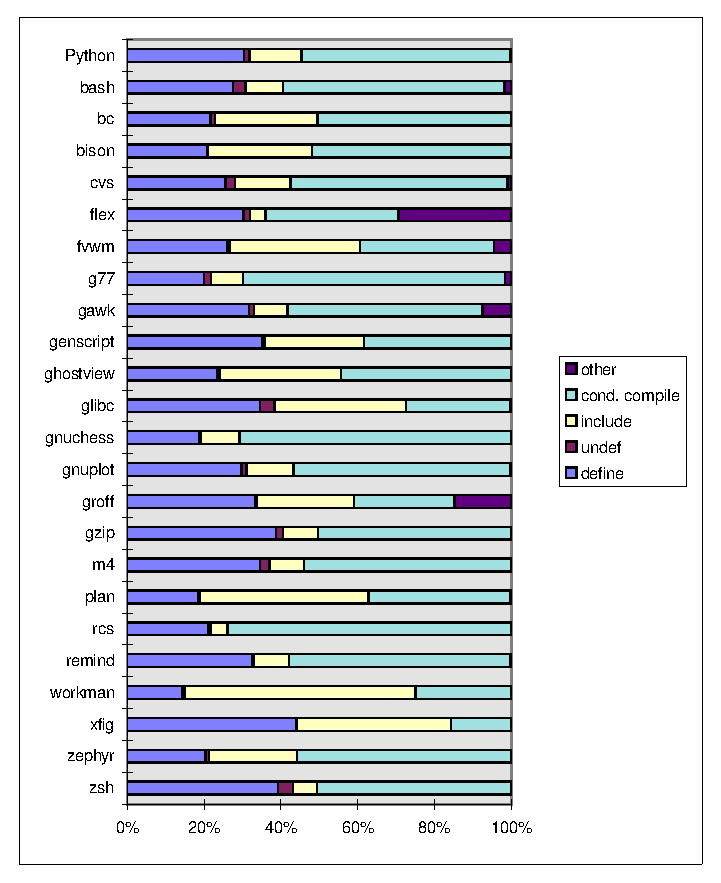
\epsfig{file=directives-breakdown.eps,height=7.5in}}
\caption{Preprocessor directives as a fraction of non-comment,
  non-blank (NCNB) lines.}
\label{fig:directives-breakdown}
\end{figure}

Overall, more than 10\% of NCNB program lines are preprocessor directives;
the percentage varies by a factor of five across packages.  Half of
the packages
have directives for over 9\% of their lines, and one in nine exceed 21\%,
indicating quite heavy use of the preprocessor.

% Figure~\ref{fig:total_directives} presents the same data arranged by
% package, to show the percentage of the total directive count attributed to
% each category of directives.

% package other   line    cond.   include undef   define  total
% Average 0.028   0.169   4.661   1.944   0.202   3.080   10.084
% (mapcar (lambda (x) (/ x 10.084)) '(0.028 0.169 4.661 1.944 0.202 3.080))

Conditional compilation directives account for just under half (46\%) of
the total directives in all packages, macro definitions comprise another
31\%, file inclusion is 19\%, macro undefinition makes up 2\%, and the
other directives are in the noise.  The directive breakdown varies by quite
a bit across packages: the percentage of {\tt \#define} varies from 14\% to
51\%, the percentage of {\tt \#include}s varies from 4\% to 60\%, and the
percentage of conditional directives varies from 16\% to 74\%.



\subsection{{\tt \#line}, {\tt \#undef}, and ``other'' directives}

The definedness of a macro is often used as a boolean value.  However, our
study shows that {\tt \#undef} is rarely used to set such macros to
``false''$\!$.  Most uses of {\tt \#undef} immediately precede a definition of
the just-undefined macro, to avoid preprocessor warnings about incompatible
macro redefinitions.  (About 90\% of \pkg{glibc}'s {\tt \#undef}s are used this
way, and 216 of the 614 {\tt \#undef}s appear in a single file which
consists of a long series of {\tt \#undef}s followed by a single {\tt
\#include}.)

Every use of {\tt \#line} (in \pkg{bash}, cvs, \pkg{flex}, \pkg{fvwm},
\pkg{gawk}, \pkg{groff}, and \pkg{perl}) appears in lex or yacc output
that enables packages build on systems lacking lex, yacc, or their
equivalents.  For instance, \pkg{flex} uses itself to parse its input,
but also includes an already-processed version of its input
specification (that is, C code corresponding to a {\tt .l} file) for
bootstrapping.

The only significant user of ``other'' directives is the \pkg{g77} package, which
contains 154 uses of {\tt \#error} (representing 1.5\% of all preprocessor
directives and 0.16\% of all lines) to check for incompatible preprocessor
flags.


\subsection{Packages with heavy preprocessor use}

Four packages\,---\,\pkg{gzip}, \pkg{glibc}, \pkg{remind}, and \pkg{bash}\,---\,deserve special
attention for their heavy preprocessor usage.  The first three have
preprocessor directives as 21--23\% of their lines.

\pkg{gzip} {\tt \#define}s disproportionately many macros as literals used as
arguments to system calls, enumerated values, directory components, and
more.  These macros act like {\tt const} variables and are evidence of good
programming style.  \pkg{gzip} also contains many conditional compilation
directives, since low-level file operations (such as setting creation time
and access control bits, accessing directories, and so forth) are done
differently on different systems; \pkg{gzip} is a highly portable program.

\pkg{glibc}'s heavy preprocessor use is largely accounted for by {\tt
  \#include} directives.  Its files' average length is just 42 NCNB
lines, and most contain several {\tt \#include} directives.  Of the
1684 files, 182 are header files consisting of a single {\tt \#include}
line, relieving \pkg{glibc} users of the need to know in which directory
a header file actually really resides.

\pkg{remind} supports speakers of many different languages by using {\tt
\#define}d constants for basically all user output.  It also contains
disproportionately many conditional compilation directives; over half of
these test the definedness of \verb|HAVE_PROTO|, in order to provide both
K\&R and ANSI prototypes.

Like \pkg{gzip}, \pkg{bash} is portable across a large variety of
systems, but \pkg{bash} uses even more operating system services.
Ninety-seven percent of \pkg{bash}'s conditional compilation directives
test the definedness of a macro whose presence or absence is a boolean
flag indicating whether the current system supports a specific feature.
The presence or absence of a feature requires different (or sometimes
additional) system calls or other code.


\section{Frequency of macro definition and usage}
\label{sec:usage}

% The second question we asked was: where and how often are macros
% defined and used in practice?  

%Specifically, for each macro we
%determined:
%\begin{itemize}\itemsep 0pt \parskip 0pt
%
%\item How many times it was {\tt \#define}d.
%\item How many times it was {\tt \#undef}ed.
%\item How many arguments (if any) it takes.
%\item How many times (and where) it was mentioned in C source code.
%\item How many times (and where) it was mentioned in other
%preprocessor directives.
%
%\end{itemize}
%[FIX: gjb: This is redundant with the same information in paragraph
%form, above]

%[FIX: gjb: I'd also like to see info about how often define-d to the same
%expansion, or not, etc.]

% \begin{figure}
% {\small
%   \setlength{\tabcolsep}{.25em}
%   \centerline{\begin{tabular}{|l|r|r|r|r|r|r|r|r|r|r|r|r|r|}\hline
\# Definitions & Python & bash & bc & bison & cvs & flex & fvwm & g77 & gawk & genscript & ghostview & glibc\\\hline\hline
1 & 71.86 & 21.52 & 53.25 & 63.21 & 34.60 & 41.10 & 55.21 & 83.45 & 40.37 & 75.19 & 50.35 & 19.46\\\hline
2 & 84.48 & 34.49 & 100.00 & 87.74 & 66.09 & 85.21 & 82.00 & 93.52 & 70.82 & 89.15 & 75.89 & 52.14\\\hline
3 & 89.93 & 39.85 & 100.00 & 87.74 & 78.31 & 87.47 & 89.24 & 95.83 & 79.82 & 89.15 & 90.78 & 68.57\\\hline
4 & 92.36 & 48.12 & 100.00 & 91.51 & 86.05 & 90.48 & 90.12 & 96.59 & 81.66 & 92.25 & 96.45 & 75.47\\\hline
5 & 94.18 & 51.88 & 100.00 & 91.51 & 87.78 & 94.24 & 90.67 & 96.83 & 82.24 & 92.25 & 100.00 & 79.95\\\hline
6 & 96.36 & 54.70 & 100.00 & 91.51 & 88.60 & 97.24 & 90.67 & 96.83 & 82.93 & 92.25 & 100.00 & 84.32\\\hline
7 & 96.79 & 55.69 & 100.00 & 91.51 & 89.57 & 97.24 & 92.97 & 98.18 & 82.93 & 92.25 & 100.00 & 86.58\\\hline
8 & 97.76 & 56.44 & 100.00 & 91.51 & 90.12 & 97.24 & 93.85 & 98.94 & 83.85 & 92.25 & 100.00 & 90.28\\\hline
9 & 98.30 & 57.28 & 100.00 & 100.00 & 90.12 & 97.24 & 94.84 & 98.94 & 85.93 & 92.25 & 100.00 & 91.16\\\hline
10+ & 100.00 & 100.00 & 100.00 & 100.00 & 100.00 & 100.00 & 100.00 & 100.00 & 100.00 & 100.00 & 100.00 & 100.00\\\hline
\multicolumn{12}{c}{} \\
\hline
\# Definitions & gnuchess & gnuplot & groff & gzip & m4 & plan & rcs & remind & workman & xfig & zephyr & zsh\\\hline\hline
1 & 67.10 & 69.76 & 33.06 & 35.48 & 32.82 & 72.55 & 56.83 & 35.61 & 68.33 & 86.69 & 61.31 & 78.79\\\hline
2 & 78.06 & 82.35 & 75.86 & 70.40 & 72.36 & 96.08 & 83.06 & 38.87 & 91.67 & 91.72 & 88.82 & 94.64\\\hline
3 & 89.68 & 86.38 & 85.14 & 79.78 & 75.24 & 98.43 & 91.26 & 42.45 & 91.67 & 93.61 & 92.67 & 96.39\\\hline
4 & 96.13 & 90.51 & 92.27 & 86.40 & 87.52 & 100.00 & 95.63 & 45.49 & 91.67 & 94.03 & 94.22 & 97.32\\\hline
5 & 96.13 & 92.57 & 92.27 & 90.99 & 88.48 & 100.00 & 95.63 & 46.58 & 100.00 & 95.60 & 94.86 & 97.32\\\hline
6 & 100.00 & 93.81 & 98.69 & 94.30 & 89.64 & 100.00 & 95.63 & 46.58 & 100.00 & 96.23 & 95.63 & 97.32\\\hline
7 & 100.00 & 94.53 & 98.69 & 98.16 & 89.64 & 100.00 & 95.63 & 49.62 & 100.00 & 96.23 & 95.63 & 97.32\\\hline
8 & 100.00 & 95.36 & 98.69 & 98.16 & 89.64 & 100.00 & 100.00 & 49.62 & 100.00 & 96.23 & 96.66 & 97.32\\\hline
9 & 100.00 & 95.36 & 98.69 & 98.16 & 91.36 & 100.00 & 100.00 & 50.60 & 100.00 & 96.23 & 96.66 & 97.32\\\hline
10+ & 100.00 & 100.00 & 100.00 & 100.00 & 100.00 & 100.00 & 100.00 & 100.00 & 100.00 & 100.00 & 100.00 & 100.00\\\hline
\end{tabular}
% Local Variables: 
% mode: latex
% TeX-master: "paper"
% End: 
}%
% }
% \caption{Number of definitions per Cpp identifier.  The numbers in the
%   table represent the percentage of identifiers which are defined a given
%   number of times or fewer.  For example, \pkg{bison} contains 4 or fewer
%   definitions for 91.51\% of all Cpp macros it defines, and no
%   macro is defined 5, 6, 7, 8, or more than 9 times.}
% \label{fig:define_count}
% \end{figure}

\begin{figure}
\centerline{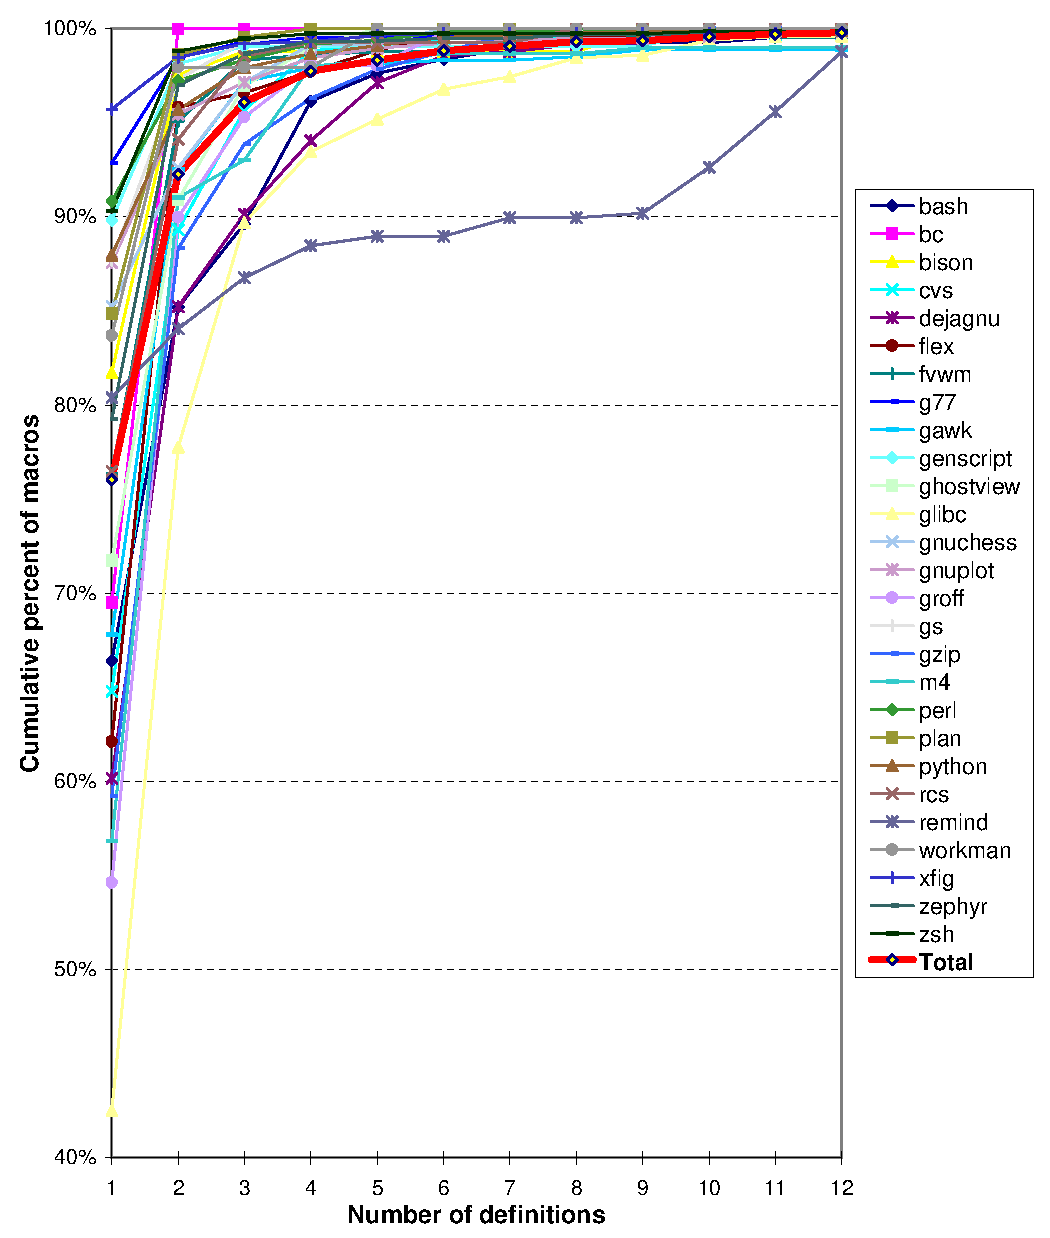
\epsfig{file=def-frequency.eps,height=7.2in}}
\caption{Number of definitions per Cpp identifier, graphed as
  the percentage of identifiers that are defined a given number of times
  or fewer.  Overall, 96\% of macros were defined three or
  fewer times; the other 4\% of macros had four or more distinct
  definitions ({\tt \#define} directives).  The outlier, for which 10\% of
  macros are defined more than eight times, is the \pkg{remind}
  package, which uses macros for all user output.}
\label{fig:freq-def}
\end{figure}

Figure~\ref{fig:freq-def} graphs the number of times each identifier is
{\tt define}d in each of the packages.  No distinction is made between
sequential redefinitions of a macro and multiple definitions that cannot
take effect in a single configuration (say, because they appear in
different branches of a Cpp conditional).

This graph shows a great deal of variation.  For example, all macros
defined by \pkg{bc} have only one or two different expansions, but more than 10\%
of macros defined by \pkg{remind} expand to more than eight different texts.

In all but four packages, at least 93\% of all macros are defined three or
fewer times.  For \pkg{bash}, \pkg{glibc}, and \pkg{dejagnu}, such macros account for 90\%,
largely because these packages are highly portable and also quite dependent
on system libraries.  The \pkg{remind} program uses macro definitions to provide
localization support for ten different natural languages (and multiple
character sets for some of them), accounting for its surprisingly large
number of macros with many definitions.  All of \pkg{remind}'s macros are defined
14 or fewer times, but 16 macros in the {\numpackages} packages are defined
more than 16 times, including three with more than 30 distinct definitions.

These data demonstrate that multiple definitions of symbols is not
numerically frequent; even more importantly, the definitions of a symbol
tend to be compatible, as shown in section~\ref{sec:categorization}.


\begin{figure}
% {\small
%   \setlength{\tabcolsep}{.25em}
%   \centerline{\begin{tabular}{|l|c|c|c|c|c|c|c|c|c|c|c|c|c|}\hline
\#Uses & bc & bison & cvs & fvwm & genscript & gnuchess & gnuplot & gzip & plan & remind & workman & xfig & zsh\\\hline\hline
0 & 6.78 & 6.10 & 7.44 & 6.53 & 1.85 & 4.51 & 39.64 & 10.12 & 4.13 & 4.66 & 0.00 & 4.05 & 2.26\\\hline
1 & 18.64 & 14.63 & 24.97 & 33.28 & 20.37 & 25.82 & 56.61 & 33.13 & 23.39 & 32.84 & 34.69 & 44.44 & 18.73\\\hline
2 & 37.29 & 30.49 & 42.38 & 49.85 & 39.81 & 41.80 & 70.60 & 52.45 & 47.71 & 53.19 & 55.10 & 58.45 & 38.38\\\hline
3 & 47.46 & 53.66 & 51.38 & 57.75 & 53.70 & 51.64 & 79.02 & 65.64 & 56.88 & 61.03 & 63.27 & 66.32 & 49.93\\\hline
4 & 57.63 & 65.85 & 59.06 & 66.72 & 60.19 & 59.02 & 83.42 & 73.31 & 61.47 & 69.85 & 65.31 & 71.41 & 58.43\\\hline
5 & 69.49 & 73.17 & 66.03 & 71.43 & 66.67 & 63.11 & 87.31 & 78.83 & 65.60 & 75.25 & 71.43 & 73.84 & 65.21\\\hline
6 & 71.19 & 76.83 & 69.75 & 76.44 & 73.15 & 65.98 & 90.03 & 81.60 & 76.15 & 79.90 & 73.47 & 77.31 & 70.52\\\hline
8 & 74.58 & 79.27 & 75.15 & 80.24 & 75.93 & 72.13 & 91.84 & 88.65 & 82.57 & 83.33 & 77.55 & 82.18 & 78.49\\\hline
10 & 77.97 & 82.93 & 79.83 & 84.04 & 80.56 & 77.46 & 93.26 & 92.02 & 87.16 & 86.76 & 81.63 & 86.81 & 83.13\\\hline
20 & 84.75 & 95.12 & 90.16 & 93.77 & 88.89 & 86.07 & 95.85 & 96.93 & 93.58 & 93.63 & 87.76 & 93.17 & 91.50\\\hline
40 & 89.83 & 96.34 & 95.44 & 97.26 & 95.37 & 91.80 & 97.28 & 98.47 & 98.17 & 95.83 & 93.88 & 96.88 & 97.74\\\hline
80 & 98.31 & 97.56 & 97.48 & 98.63 & 98.15 & 95.90 & 98.58 & 99.39 & 98.62 & 97.79 & 95.92 & 98.73 & 99.47\\\hline
$>$80 & 100.00 & 100.00 & 100.00 & 100.00 & 100.00 & 100.00 & 100.00 & 100.00 & 100.00 & 100.00 & 100.00 & 100.00 & 100.00\\\hline
%\hline
\end{tabular}
% Local Variables: 
% mode: latex
% TeX-master: "paper"
% End: 
}%
% }
\centerline{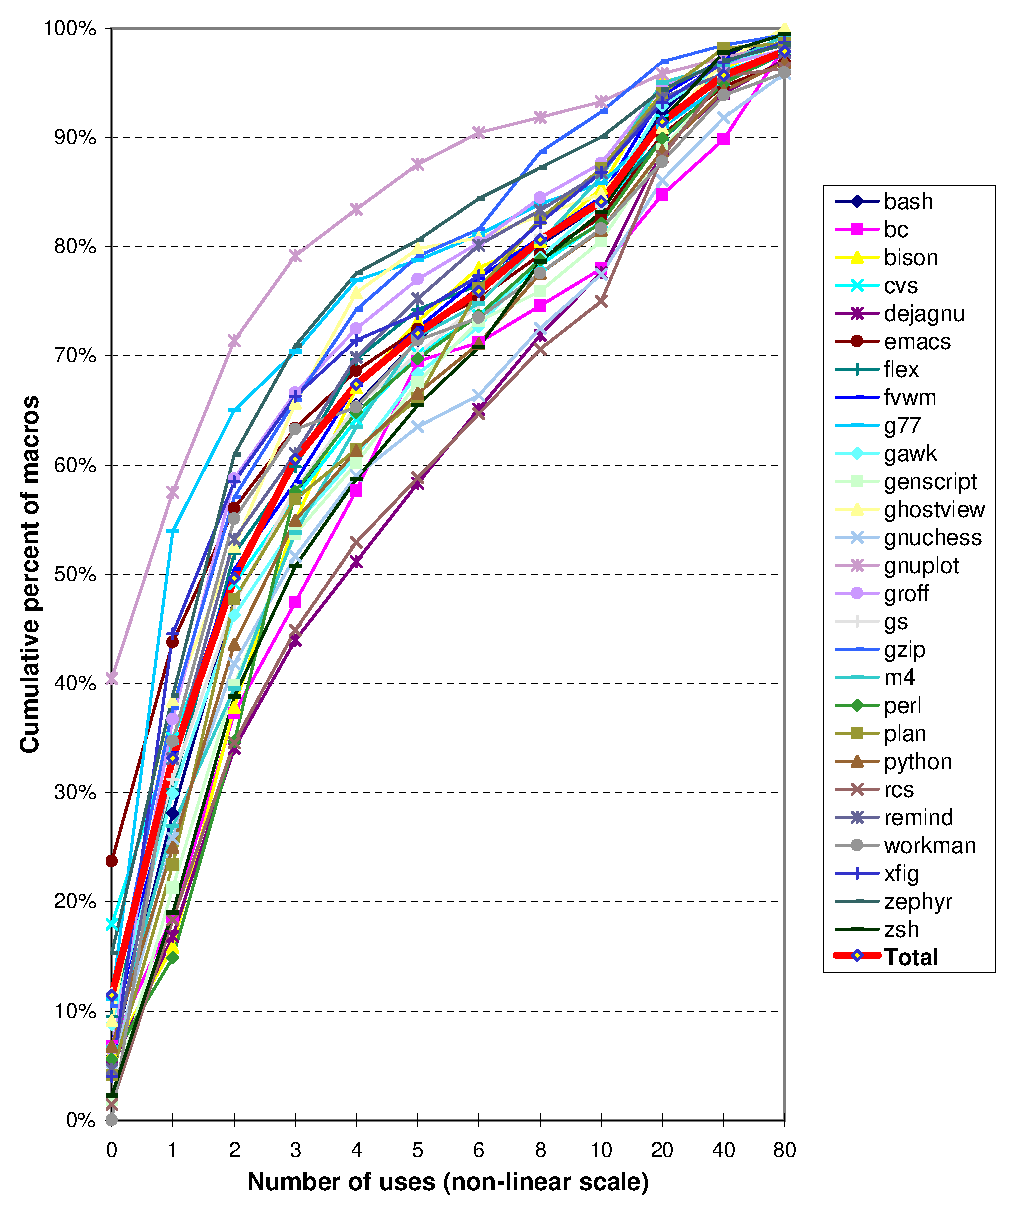
\epsfig{file=use-frequency.eps,height=7.5in}}
\caption{Number of expansions per Cpp macro.  The numbers in the
  table represent the percentage of identifiers which are expanded a given
  number of times or fewer.  For example, \pkg{g77} expands 65\% of its
  macros two or fewer times.}
\label{fig:freq-use}
\end{figure}

Figure~\ref{fig:freq-use} is structured as the previous figure, but it
represents the number of times that a defined name is expanded in either
the package (not in system headers).  About 82\% of all macros were
expanded eight or fewer times.

It is notable that most packages contain a significant number of defined
macros that are never expanded\,---\,on average, over 13\%.
(Figure~\ref{fig:freq-use} reports only on macros defined in a package, not
those defined in system or library header files, inclusion of which would
push the unused percentage well above 50\%.)  Most packages are in the
4-12\% range, while \pkg{gnuplot} exceeds 40\%.  Although it's difficult to fully
account for the larger numbers, contributing factors include a lot of
cut-and-paste and a lack of attention to implementations for specific
platforms in some packages.  Macros with 10 or fewer uses cover
approximately 85\% of the cases.

The tail of this distribution is quite long, indicating that some macros
are used very heavily.  Ninety-nine percent of macros are expanded 147 or fewer
times, 99.5\% of macros are expanded 273 or fewer times, 99.9\% are
expanded 882 or fewer times, and \pkg{python} uses {\tt NULL} (which \pkg{python}
itself defines) 4233 times.  Figure~\ref{fig:freq-use} weights each macro
equally rather than weighting each macro use equally, which would weight
\pkg{python}'s {\tt NULL} 4233 times more heavily than a macro used only once
(and infinitely more than a macro never used at all).  Only macros defined
in a package, and uses in that package, are counted; system macros and uses
are excluded.


\begin{figure}
\centerline{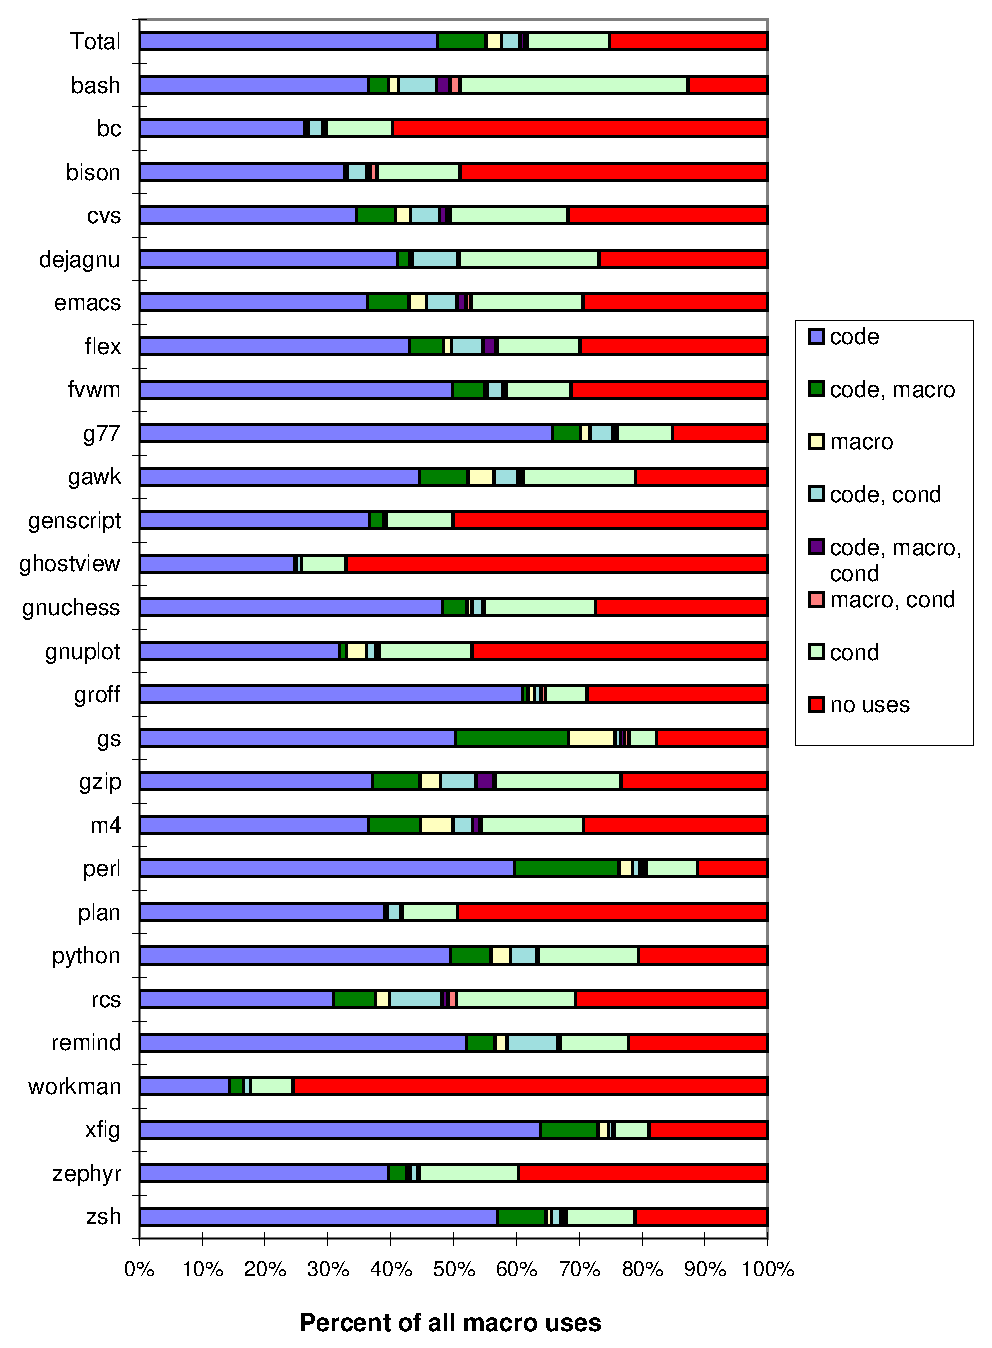
\epsfig{file=where-used.eps,height=6in}}
%{\small
%  \setlength{\tabcolsep}{.25em}
%  \begin{tabular}{|l|r|r|r|r|}\hline
Package & CodeOnly & CppAndCode & CppOnly & NoUses\\\hline
Python & 861 & 166 & 193 & 100\\\hline
bash & 348 & 84 & 147 & 59\\\hline
bc & 43 & 6 & 2 & 19\\\hline
bison & 62 & 6 & 6 & 17\\\hline
cvs & 401 & 137 & 128 & 59\\\hline
flex & 162 & 46 & 26 & 40\\\hline
fvwm & 489 & 77 & 42 & 55\\\hline
gawk & 265 & 103 & 48 & 33\\\hline
genscript & 76 & 7 & 18 & 17\\\hline
gnuchess & 190 & 28 & 8 & 26\\\hline
gnuplot & 303 & 39 & 97 & 319\\\hline
groff & 420 & 14 & 18 & 42\\\hline
gzip & 144 & 82 & 50 & 19\\\hline
m4 & 122 & 44 & 30 & 20\\\hline
plan & 194 & 11 & 3 & 24\\\hline
rcs & 55 & 68 & 9 & 17\\\hline
remind & 293 & 52 & 41 & 32\\\hline
workman & 36 & 9 & 1 & 16\\\hline
xfig & 678 & 105 & 25 & 45\\\hline
zephyr & 354 & 46 & 63 & 96\\\hline
zsh & 590 & 84 & 24 & 31\\\hline
\end{tabular}
%
%}
\caption{Where macros are used: in C code, in macro definition bodies, in
  conditional tests, or in some combination thereof.  The figure reflects
  only package macros and uses, not system files.}
\label{fig:where-used}
\end{figure}

Figure~\ref{fig:where-used} breaks down macro usage according to whether
the macro invocation occurs in Cpp directives (which is further broken
down into conditional tests and definition bodies), in other C code, in
both, or in neither (i.e., no uses).

No package expanded all of its defined macros; two expanded fewer than 70\%
of the defined macros.  The dominant usage was in C code only; these uses
do not, therefore, have any affect on conditional compilation (for example).

In general, packages use macros either to direct conditional compilation or
to produce code, but not for both purposes; this separation of concerns
makes the source code easier to understand.  Only 3.1\% of macros expand in
both code and conditional contexts (the fourth and fifth categories in the
figure; the sixth, macro and conditional, accounts for only another 0.2\%
of macros). 
Conditional usage is rare in general; conditional compilation accounts for
half of Cpp directives but only 5.4\% of macros (plus the categories just
listed above).



\section{Categorization}
\label{sec:categorization}

This section examines the purposes of macros and how they are intended to
be used, which requires heuristic categorization of macro definition bodies.  A
straightforward refinement that we are pursuing examines macro uses to aid
this categorization.  (For example, a macro used where a type should appear
can be inferred to expand to a type; a macro used before a function body is
probably expanding to a declarator.)

In addition to classifying each macro as taking arguments or not, our tool
identifies the following specific categories (and a number of more
rarely-used ones omitted for brevity;
figure~\ref{fig:subset-categories} contains a more complete list).  The examples
are chosen for clarity and brevity from the packages studied.

\begin{description}
  \sloppy
  \emergencystretch=2em

\item[Null define]  The {\tt \#define} gives only an
  identifier name but no macro body, as in {\tt \#define
  \verb|HAVE_PROTO|}\@.  Such macros appear most frequently in Cpp
directives (such as {\tt \#ifdef}), where they are used as boolean
variables by the preprocessor, but may also appear in code.  For instance,
macro {\tt private} may expand either to {\tt static} or to nothing,
depending on whether a debugging mode is set.  The definition which
causes it to expand to nothing is categorized as a null define (the
other is categorized as ``other syntactic macro'';  see below).

\item[Constant] The macro is defined to be either a literal or an operator
  applied to constant values.  For instance, {\tt \#define NULL 0}, {\tt \#define
  \verb|ARG_MAX| 131072}, and {\tt \#define ETCHOSTS "/etc/hosts"} define
literals, while {\tt \#define \verb|RE_DUP_MAX| ((1<<15)-1)} and {\tt
\#define \verb|RED_COLS| (1 << \verb|RED_BITS|)} (where \verb|RED_BITS| is
a constant, possibly a literal) define constants.  Such macros act like
{\tt const} variables.

\item[Expression]  The macro body is an expression, as in {\tt \#define
  sigmask(x) (1 << ((x)-1))}.  This expression might have a single constant
value everywhere (the usual case for expression macros without arguments,
most of which are classified as constants, above) or might have a
different value on each use (the usual case for expression macros with
arguments).

One tenth of expression macros in our study use assignment operators, which
have potentially unexpected results.  A macro argument that is assigned to
is similar to a pass-by-reference function argument and need only be noted in the
macro's documentation.  A macro that assigns a global variable also
presents no difficulties in understanding or translation into a C++
inline function.
Assignment to a local variable that is free in the macro body, however,
demands that such a variable exist wherever the macro is invoked, and
assigns to different variables at different invocations.\footnote{By
  contrast, LCLint considers assignment to a macro argument dangerous but
  does not appear to check for assignments to local
  variables.~\cite{Evans:LCLint}} Such a macro implements a restricted form
of dynamic scoping by capturing the instance of a variable visible at
the point of macro invocation.

% Computed ``10\% use assignment'' from CATEGORIES_NI lines of *.stat files.

% Problem: can't figure out how to get typewriter curly braces in footnote.
\item[Statement]  The macro body is a complete statement such as
  ``{\tt x = 3;}'', ``{\tt if (s) free(s);}'' or ``{\tt \verb|{| int x =
    y*y; printf("\%d", x); \verb|}|}''.  Such a macro is like a function
    returning {\tt void}, except that uses should not be followed by a
    semicolon.\footnote{Since the body is already a complete statement, the
      extra semicolon can cause problems such as mis-parsing of nested {\tt
      if} statements.  Such macros can be confusing to use, because
    programmers are inclined to add a semicolon after invocations that look
    like functions; wrapping the body in {\tt do \{\ldots\} while (0)}, a
    partial statement which requires a trailing semicolon, solves this
    problem.  To our surprise, we found few uses of that construct, but
    many error-prone instances of a macro that expanded to a statement like
    \{\ldots\} in which a call to the macro was immediately followed by a
    semicolon.}

\item[Stringization and pasting]  The macro body contains {\tt \#} or
  {\tt \#\#}, which treat the macro argument not as a token but as a
  string.  Examples include {\tt \#define spam1(OP,DOC) \verb|{|\#OP, OP,
    1, DOC\verb|}|,}, {\tt \#define REG(xx) register long int xx asm
    (\#xx)}, and {\tt \#define \verb|__CONCAT|(x,y) x \#\# y}.  No C or C++
  language mechanism can replace such macros.

\item[Other syntactic macros]  Like stringization and pasting, these
  macros make essential use of the unique features of the preprocessor.
  Our framework separately categorizes a number of such macros, including
  those that expand to a reserved word (such as {\tt \#define private
  static}, mentioned above), those that expand to a delimiter (such as
{\tt \#define AND ;}), and those with mismatched parentheses, brackets, or
braces.  The latter are often used to create a block and perform actions
that must occur at its beginning and end, as for \verb|BEGIN_GC_PROTECT|
and \verb|END_GC_PROTECT|.

\item[Type-related macros]  These macros either take a type as an argument, pass
  a type to another macro, expand to a type or partial type, or use such a
  macro.  Examples include {\tt \#define \verb|__ptr_t| void *}, {\tt
  \#define \verb|__INLINE| extern inline}, {\tt \#define \verb|ALIGN_SIZE|
sizeof(double)}, and {\tt \#define PTRBITS \verb|__BITS|(char*)}.  Since
types are not first-class in C, they may not be passed to functions or
returned as results; additionally, these macros may produce or use only
part of a type (such as a storage class).  As a result, these macros may be
tricky to understand, and cannot be eliminated via straightforward
translation (though C++ templates may provide some hope).

\item[Recursive]  The ISO C standard permits macros to be recursively
  defined (the preprocessor performs only one level of expansion), as in
  {\tt \#define LBIT vcat(LBIT)}.  This mechanism permits already-defined
  or to-be-defined macros to be extended or modified.

\item[Classification failure]  Multiple adjacent identifiers\,---\,as in
  {\tt \#define EXFUN(name, proto) name proto} and {\tt \#define
  \verb|DO_OP|(OP,a,b) (a OP b)}\,---\,caused many failures of our
  classification heuristics.  Of the 1025 classification failures in the
  {\numpackages} packages, 496 were caused by a single definition in
  \pkg{gnuplot}, {\tt \#define CUR \verb|cur_term->type.|} (the period is
  part of the expansion), and uses of that macro, as in {\tt \#define
  \verb|acs_plus| CUR Strings[408]}.  Four packages\,---\,\pkg{bison},
  \pkg{gnuchess}, \pkg{remind}, and \pkg{workman}\,---\,had no macro
  classification failures.  These packages contain 93, 297, 932, and 58 macro
  definitions, respectively.

% and illegal identifier
%   names ({\tt \#define \verb|FAT$C_VFC| 3} for VMS compilation), tokens %$HACK
%   ({\tt \#define \verb|LIB_PATH| /usr/ucblib}), and constants ({\tt 1ULL} for
%   {\tt unsigned long long})

%   \pkg{gnuplot}
%   contains only 13 other failures, ghostscript has 130, and no other
%   package stands out with many.

% half appeared in \pkg{gnuplot};
% \pkg{gnuplot}, cvs, and \pkg{groff} accounted for over 75\% of the failures, many of
% which could be eliminated by slightly relaxing the parsing rules.
\end{description}


Figure~\ref{fig:categorization} shows the percentage of macros that fit
into these categories for each package.  Overall, 83\% of macros are
expressions\,---\,mostly constants; further analysis of the conditional
compilation structure (in the style of Krone and Snelting~\cite{Krone94})
and of the macros with free variables (essentially achieving dynamic
scoping) is needed to see which of the roughly 33\% of expression macros
should be easy to convert to C++ language features such as constants or
enumerated values.  The 7\% that are null
defines, should also be easy to understand and/or translate.  Another 5\%
are statements, most of which are straightforward (complications include
scoping and semicolon swallowing).  That only 0.2\% of macros exploit
stringization or pasting, the only truly extra-linguistic capabilities in
the C preprocessor, is encouraging.

Our tool failed to categorize less than 2\% of the 26701 definitions;
performing even a single level of macro expansion in bodies would make most
of those failures categorizable.  Other straightforward improvements
include making a second pass after an initial categorization and using
dependence information to determine which definitions can be active at an
invocation site.  We have not pursued these enhancements, primarily because
our tool is already accurate enough for our purposes.


% The following isn't quite enough to get the columns lined up in this table.
% \newcolumntype{d}{D{.}{.}{2}}
% \begin{tabular}{|l|d|d|d|d|d|d|d|}\hline
\begin{figure}
% {\small
%   \setlength{\tabcolsep}{.25em}
%   \centerline{\begin{tabular}{|l|c|c|c|c|c|c|c|}\hline
Package & Null define & Literal & Expression & Statement & Stringization and pasting & Other syntatic macros & Failed classification\\\hline
Python & 176 & 510 & 865 & 50 & 5 & 62 & 21\\\hline
bash & 717 & 679 & 637 & 3 & 3 & 62 & 30\\\hline
bc & 4 & 36 & 37 & 2 & 0 & 9 & 1\\\hline
bison & 4 & 64 & 32 & 0 & 0 & 2 & 0\\\hline
cvs & 106 & 683 & 530 & 58 & 0 & 69 & 116\\\hline
flex & 32 & 224 & 87 & 19 & 0 & 36 & 2\\\hline
fvwm & 48 & 748 & 122 & 11 & 0 & 27 & 1\\\hline
gawk & 49 & 243 & 391 & 11 & 0 & 59 & 23\\\hline
genscript & 8 & 71 & 39 & 0 & 0 & 9 & 0\\\hline
gnuchess & 12 & 201 & 93 & 5 & 0 & 5 & 1\\\hline
gnuplot & 134 & 577 & 244 & 3 & 0 & 18 & 9\\\hline
groff & 18 & 607 & 148 & 11 & 1 & 36 & 98\\\hline
gzip & 110 & 229 & 130 & 25 & 0 & 21 & 4\\\hline
m4 & 36 & 83 & 272 & 26 & 0 & 62 & 1\\\hline
plan & 9 & 208 & 43 & 4 & 0 & 4 & 2\\\hline
rcs & 15 & 54 & 80 & 14 & 0 & 18 & 3\\\hline
remind & 11 & 744 & 108 & 65 & 0 & 18 & 2\\\hline
workman & 1 & 41 & 25 & 2 & 0 & 0 & 0\\\hline
xfig & 31 & 681 & 240 & 24 & 0 & 20 & 0\\\hline
zephyr & 80 & 451 & 255 & 28 & 0 & 27 & 2\\\hline
zsh & 31 & 520 & 267 & 20 & 0 & 40 & 5\\\hline
\hline
Total & 1632 & 7654 & 4645 & 381 & 9 & 604 & 321\\\hline
\end{tabular}}%
% }
\centerline{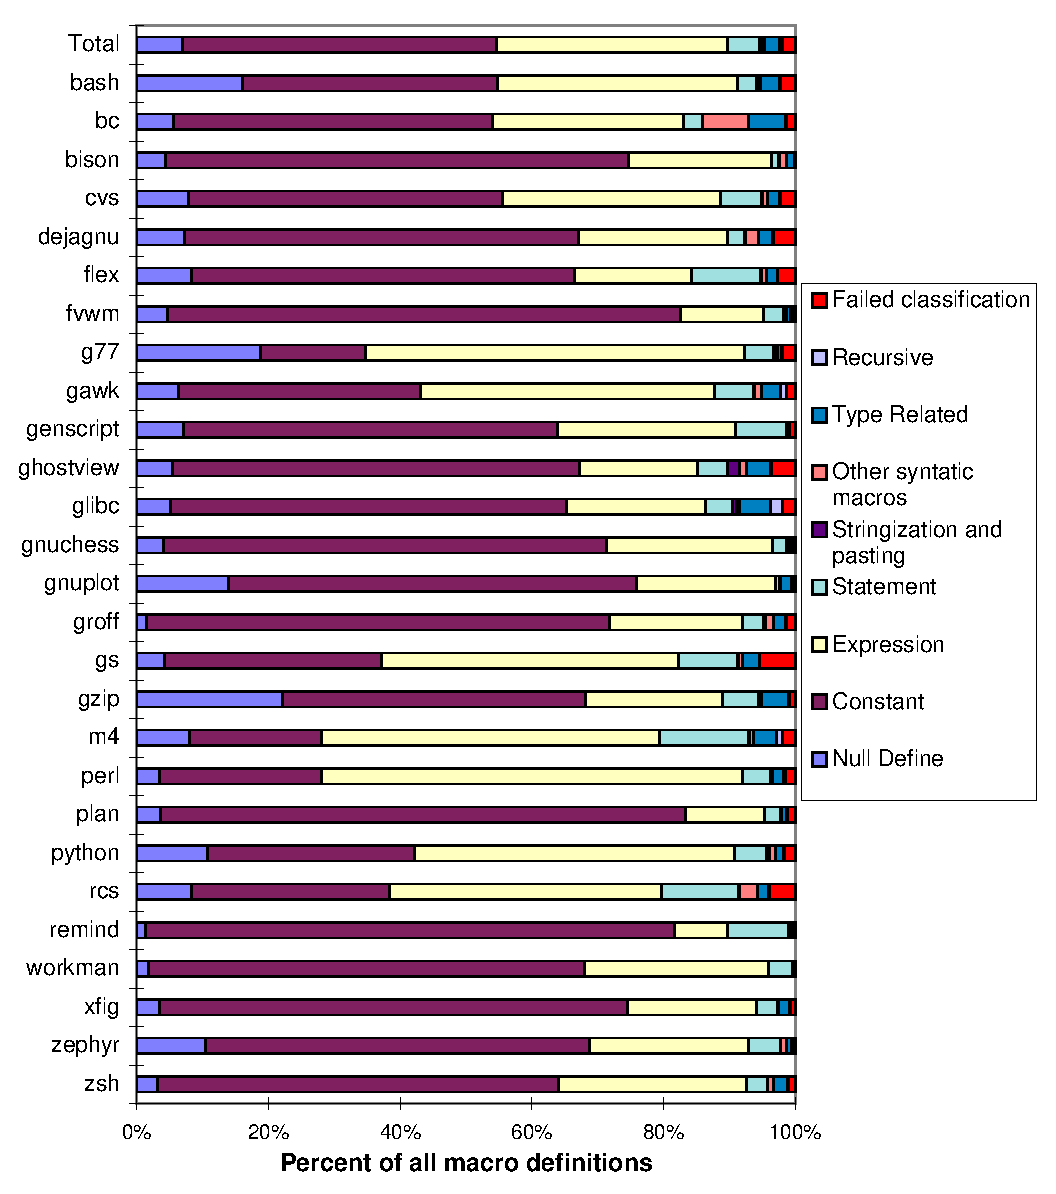
\epsfig{file=def-categories.eps,height=6in}}
\caption{Categorization of macro definition bodies.}
\label{fig:categorization}
\end{figure}



%In anticipation of the translator tool, the analysis tool infers
%types, using techniques similar to those of Siff and Reps~\cite{Siff-fse96}
%and O'Callahan and Jackson~\cite{OCallahan-icse97}.  Our use of the
%type information is in the early stages, however, and we do not report
%on the preliminary results in this paper.

% [FIX: Benefits even from simple literal constant conversion -- exposes
% symbolic information to the debugger]

%[FIX: Should this also include Mike's manual breakdown into categories
%for gzip.]


\begin{figure}
{\small\centerline{
%\usepackage{graphics}
%\newcommand{\black}{\ensuremath{\blacksquare}}
\newcommand{\black}{\vrule height5.5pt depth0.5pt width6pt}
{\small
\addtolength{\columnsep}{-.5\columnsep}
\begin{tabular}{|r|*{22}{c|}}\hline
\rotatebox{90}{Percentage of macro names} &
\rotatebox{90}{failed categorization} &
\rotatebox{90}{null define} &
\rotatebox{90}{expression} &
\rotatebox{90}{expression with assignment} &
\rotatebox{90}{expression with free variables~} &
\rotatebox{90}{literal} &
\rotatebox{90}{constant} &
\rotatebox{90}{some constant} &
\rotatebox{90}{has type argument} &
\rotatebox{90}{uses macro as function} &
\rotatebox{90}{uses macro as type} &
\rotatebox{90}{uses type argument} &
\rotatebox{90}{expands to type} &
\rotatebox{90}{expands to reserved word} &
\rotatebox{90}{statement} &
\rotatebox{90}{recursive} &
\rotatebox{90}{assembly code} &
\rotatebox{90}{expands to syntax tokens} &
\rotatebox{90}{mismatched entities} &
\rotatebox{90}{token pasting} &
\rotatebox{90}{stringization}
\\\hline
    39\% & & & & & &\black& & & & & & & & & & & & & & &  \\\hline
    34\% & & &\black& & & & & & & & & & & & & & & & & &  \\\hline
   7.3\% & &\black& & & & & & & & & & & & & & & & & & &  \\\hline
   4.2\% & & & & & & & & & & & & & & &\black& & & & & &  \\\hline
   3.7\% & & & &\black& & & & & & & & & & & & & & & & &  \\\hline
   3.6\% &\black& & & & & & & & & & & & & & & & & & & &  \\\hline
   2.4\% & & & & & & & &\black& & & & & & & & & & & & &  \\\hline
  0.64\% & & & & & & & & & & & & &\black& & & & & & & &  \\\hline
  0.46\% & &\black& & & & & & & & & & & & &\black& & & & & &  \\\hline
  0.46\% & & &\black& & &\black& & & & & & & & & & & & & & &  \\\hline
  0.39\% & & & & & & & & & & & &\black& & & & & & & & &  \\\hline
  0.36\% & & & &\black& & & & & & & & & & &\black& & & & & &  \\\hline
  0.25\% & &\black& & & &\black& & & & & & & & & & & & & & &  \\\hline
  0.24\% & &\black&\black& & & & & & & & & & & & & & & & & &  \\\hline
  0.21\% & & &\black&\black& & & & & & & & & & & & & & & & &  \\\hline
  0.19\% & & & & & & & & & & &\black& & & & & & & & & &  \\\hline
  0.18\% & &\black& & & & & & & & & & &\black& & & & & & & &  \\\hline
  0.18\% & & &\black& & & & & & & & & & & &\black& & & & & &  \\\hline
  0.14\% &\black& &\black& & & & & & & & & & & & & & & & & &  \\\hline
  0.12\% &\black&\black& & & & & & & & & & & & & & & & & & &  \\\hline
  0.12\% & & &\black& & & & & & & & & & & & & & &\black& & &  \\\hline
  0.11\% & & & & & & & & & & & & & & & & & & &\black& &  \\\hline
 0.096\% & & & & & & & & & & & & & & & &\black& & & & &  \\\hline
 0.081\% & & & & & &\black& & & & & & & & &\black& & & & & &  \\\hline
 0.076\% & & &\black& & & & &\black& & & & & & & & & & & & &  \\\hline
  0.07\% & &\black& &\black& & & & & & & & & & & & & & & & &  \\\hline
  0.07\% & & & & & & & & & &\black& & & & & & & & & & &  \\\hline
  0.06\% &\black& & & & &\black& & & & & & & & & & & & & & &  \\\hline
  0.06\% & & &\black& & & & & & & &\black& & & & & & & & & &  \\\hline
 0.055\% &\black& & & & & & & & & & & & & &\black& & & & & &  \\\hline
 0.055\% & & & & & & & &\black& & & & & & & & & &\black& & &  \\\hline
  0.05\% & & &\black& & & & & & & & & &\black& & & & & & & &  \\\hline

\end{tabular}}
}}
\caption{Subset categorization of macros (not macro definitions).   Items
  less than one twentieth of a percent are omitted; such items appear
  fewer than ten times in the codebase.}
\label{fig:subset-categories}
\end{figure}
 
Figure~\ref{fig:subset-categories} indicates that multiple definitions of a
particular macro tend to be compatible.  It classifies macros rather than
macro definitions, and uses a finer breakdown of categories.  Each macro is
given a set of categorizations (corresponding to the categorizations of its
definitions) and the incidence of each such is displayed.  For over 97\% of
macros, all of the macro's definitions are given the same
categorization\,---\,even when categories such as literal, constant,
expression, and expression with assignment are considered unrelated.  The
most common ``conflict'', statement and null define, is also harmless in
most contexts.  We expect that closer examination of most of the other
conflicts will demonstrate that they present no real obstacles to
understanding (even if they do complicate some details).


\section{Conclusions}
\label{sec:conclusion}

% \subsection{Who cares?}
\subsection{Relevance of the results}

The results of this research are of interest to language designers, tool
writers, programmers, and software engineers.

Language designers can examine uses of the macro system's extra-linguistic
capabilities to determine what programmers consider missing from the
language.  Future language specifications can support (or prevent!)\ such
practices in a more disciplined, structured way.

% [[[Think more about this:  Also, how do language choices lead to more/less
% tightly integrated (as opposed to open, component-based) environments?
% E.G., no need for \verb|__LINE__| in Java?]]]

Programming tool writers, too, need to understand how Cpp is used, for that
sheds insight on the sorts of inputs that will be provided to the tool.  By
coping with the most common constructs, the tool can provide relatively
good coverage for low effort.  By identifying problematic uses, much better
feedback can be given to the programmer, who can be more effective as a
result.  The analysis results also indicate the difficulty of processing
preprocessor directives; before these analyses, we did not know whether the
task was so trivial as to be uninteresting, so difficult as to be not worth
attempting, or somewhere in between.

The analyses are of interest to programmers who wish to make their code
cleaner and more portable, and can help them to avoid constructs that cause
tools (such as test frameworks and program understanding tools)
to give incomplete or incorrect results.

% Also, learn weird new Cpp tricks!

Finally, our results are of interest to software engineers for all of the
above reasons and more.  Since this is the first Cpp usage study of which
we are aware, it is worth performing simply to determine whether the
results were predictable a priori; we did in fact discover a number of
interesting features of our suite of programs.


\subsection{Making C programs easier to understand}

The combination of C and Cpp makes a source text unnecessarily difficult to
understand.  A good first step is to eliminate Cpp uses where an equivalent
C or C++ construct exists, and to apply tools to explicate the remaining
uses.  Here we discuss a few approaches to solving this problem by
eliminating the source of confusion rather than applying tools.  We do not
seriously consider simply eliminating the preprocessor, for it provides
conveniences and functionality not present in the base language.

Since many of the most problematic uses of Cpp provide portability across
different language dialects or different operating environments,
standardization can obviate many such uses.  Canonicalizing library
function names and calling conventions makes conditional compilation less
necessary and incidentally makes all programs more portable, even those
which have not gone to special effort to achieve portability.  This
proposal moves the responsibility for portability (really, conformance to a
specification) from the application program into the library or operating
system, which is a reasonable design choice since many application programs
rely on a much smaller number of libraries and run on relatively few
operating systems.

Likewise, the most common single cause for Cpp directives would be
eliminated if the C language and its dialects had only a single declaration
syntax.  Because most C compilers, and all C++ compilers, accept ANSI-style
declarations, much support for multiple declaration style may have outlived
its usefulness.  We are investigating the effect on our statistics (and
program understandability) of ``partially evaluating'' a program source by
specifying the definedness and values of some Cpp identifiers.

Some Cpp directives, such as {\tt \#include}, can be moved into the
language proper; this would also eliminate the need for Cpp constructs that
prevent multiple inclusion of header files.  Likewise, compilers that do a
good job of constant-folding and dead code elimination can encourage
programmers to use language constructs rather than relying on the
guarantees of an extra-linguistic tool like Cpp.\footnote{Interestingly,
  the issue seems to not be whether compilers do the appropriate
  optimizations, but whether programmers have confidence that the
  optimizations will be performed; if unsure, programmers will continue to
  resort to Cpp, since certainly a compiler cannot generate code for source
  that it does not ever even see (because Cpp has already stripped it
  away).}

Common Cpp constructs could be replaced by a special-purpose syntax.  For
instance, declarations or partial declarations could be made explicit
(perhaps first-class) objects; similar support could be provided for
repetitive constructs and dynamic scoping.  Manipulations of these objects would then
be performed through a clearly-specified interface rather than via string
concatenation, easing the understanding burden on the programmer.  Such
uses would also be visible to the compiler and could be checked and
reasonable error messages provided.  The downside of this approach is the
introduction of a new syntax or new library functions which may not
simplify the program text and which cannot cover all cases, only a few
specified ones.

An alternative approach which avoids the clumsiness of a separate language
of limited expressibility is to make the macro language more
powerful\,---\,perhaps even using the language itself via constructs
evaluated at compile time rather than run time.  (The macro systems of
Common Lisp and Scheme, and their descendants~\cite{WeiseC93}, take this
approach.)  An extreme example would be to provide a full-fledged
reflection capability.  Such an approach is highly general, powerful, and
and theoretically clean; it circumvents many of the limitations of Cpp,
though it does not necessarily support all of Cpp's low-level features.
However, this approach may degrade rather than improve programs
understanding.  As difficult as it may be to determine what output a
macroless program produces, it can be just as difficult simply to determine
the text of a program which uses such macros.  (This is also a problem with
meta-object protocols, aspect-oriented programming, and intentional
programming, all of which permit the programmer to specify transformations
on other parts of the source code.  In practice, such systems are used in
fairly restricted ways, perhaps because other uses would be too
complicated.)  A dialog among users, compiler writers, tool writers, and
language theorists is necessary when introducing a feature in order to
prevent unforeseen consequences from turning it into a burden.


[[inserted from intro: surely not yet in the right place]
On the other hand, the analysis also
convinces us that, by extending our analysis framework with some class
type inferencing techniques (similar to those used by Siff and Reps
for C to C++ translation~\cite{Siff-fse96}, O'Callahan and Jackson for
program understanding~\cite{OCallahan-icse97}, and others), we can
take significant steps towards a tool that usefully converts a high
percentage of Cpp code into C++ language
features.\footnote{Preliminary results indicate that many C++ packages
rely heavily on Cpp, even when C++ supports a nearly identical
language construct, probably due to a combination of trivial
translations from C to C++ and of C programmers becoming C++
programmers without changing their habits.} We are interested not in
translations that merely allow a C program to be compiled by a C++
compiler (which is usually easy, by intentional design of C++) but
those that take advantage of the added richness and benefits of C++
constructs.

All three approaches would be unnecessary if programs did not use
preprocessor directives.  This is exactly what Stroustrup suggests:
\begin{quote}
  I'd like to see Cpp abolished.  However, the only realistic and
  responsible way of doing that is first to make it redundant, then
  encourage people to use the better alternatives, and {\em then\/}\,---\,years
  later\,---\,banish Cpp into the program development environment with the
  other extra-linguistic tools where it
  belongs~\cite[p.~426]{Stroustrup-DesignEvolution}.
\end{quote}
C++ contains features\,---\,such as constant variables, inline functions,
templates, and reference parameters\,---\,that obviate many uses of Cpp.
Thus, translation to C++ is a path for partial elimination of Cpp.

This study indicates the feasibility\,---\,and our framework for
analyzing preprocessor usage provides a basis for the
development\,---\,of an automatic translator with two attractive
properties.  It would take as input C programs complete with
preprocessor directives, and it would map many\,---\,preferably
most\,---\,uses of directives into C++ language features.  (It is not
practical to eliminate all uses of Cpp.  For example, C++ currently
provides no replacement for the {\tt \#include} directive, or for
stringization or pasting.  Macros that cannot be eliminated might be
annotated with their types or effects on parser or program state, so
that even tools that do no Cpp analysis can operate correctly on such
programs.)

]]



%% See slide 15 and its notes from Mike's quals talk.
% \subsection{Future work}
% 
% These results suggest a wide variety of future avenues for research, both
% in terms of expanding our understanding of uses of the preprocessor in
% practice and in addressing the issues identified by this study.


\section{Related work}
\label{sec:related}

We could find no other empirical study of the use of the C preprocessor nor
any other macro processor.  However, we did find guidance on using C macros
effectively and tools for checking macro usage.

Carroll and Ellis state that ``almost all uses of macros can be eliminated
from C++ libraries''~\cite[p.~146]{Carroll95}.  They list eight categories
of macro usage and explain how to convert them into C++ mechanisms.  They
do not discuss automatic conversion, but focus on instructing the software
engineer on better ways to do Cpp-like things.

Similarly, a number of organizations provide hints about effective ways to
the use the C preprocessor.  The GNU documentation, for example, discusses
a set of techniques including simple macros, argument macros, predefined
macros, stringization macros, concatenation macros, undefining and
redefining macros.  It also identifies a set of ``pitfalls and subtleties
of macros''; these are much like some of the problems our analysis tool
identifies.  We discovered that these categorizations sometimes focussed on
constructs that don't happen very often or missed ones that are actually
frequent.  Our effort not only categorizes problems, but it also determines
the frequency of appearance of those problems and discovers other
idiosyncratic uses.

A number of tools check whether specific C programs satisfy particular
constraints.  The lint program checker, distributed with most Unix systems,
checks for potentially problematic uses of C\@.  The implementation of lint
is complicated by the fact that it tries to replicate significant functions
of both the C compiler and the preprocessor.

LCLint performs many of lint's checks and also
allows the programmer to add annotations which enable additional
checks~\cite{Evans-pldi96,Evans-fse94}.
LCLint optionally checks function-like
macros\,---\,that is, those which take arguments\,---\,for
macro arguments on the left hand side of assignments, for statements
playing the role of expressions, and for consistent return types.
%\begin{quote}
%$\ldots$ a parameter to a macro may not be used as the left hand side
%of an assignment expression $\ldots$, a macro definition must be
%syntactically equivalent to a statement when it is invoked followed by
%a semicolon $\ldots$, the type of the macro body must match the return
%type of the corresponding function $\ldots$\footnote{From Section 8 of
%David Evans's LCLint User's Guide, Version 2.2 (August 1996); larch-www.lcs.mit.edu:8001/\discretionary{}{}{}larch/\discretionary{}{}{}lclint/\discretionary{}{}{}guide/\discretionary{}{}{}guide.html}
%[FIX: That footnote should really be a reference instead.]
%\end{quote}
%[Fix: that quotation is really easy to nitpick:
% 1) assignment parameters is fine (just turn into a reference argument) but
%    assignment of non-parameters that aren't at global scope is quite bad.
% 2) in x=foo(); we do NOT want foo() to be a statement
% 3) a macro doesn't have a single type, but may have many polymorphic types
%Should we mention these things?  I don't want to seem nitpicky or petty.]
LCLint's approach is prescriptive: programmers are encouraged not to use
constructs that might be dangerous, or to change code that contains such
constructs.  We are more interested in analyzing, describing, and
automatically removing such uses so that tools can better process existing
code without requiring human interaction or producing misleading results.

%% FIX: If we could also list the platforms for which each can compile,
%% that would be great, but I doubt the benefit is worth the effort for now

Krone and Snelting use mathematical concept analysis to determine the
conditional compilation structure of code~\cite{Krone94}.  They determine,
for each line, which preprocessor macros it depends upon, and display that
information in a lattice.  They do not determine how macros depend upon one
another directly, only by their nesting in {\tt \#if}, and the information
conveyed is about the program as a whole.


% Not really right:  Don't want the ``References'' section head to be small.
{\small \bibliography{evil}}

\end{document}
